\chapter{Технологический раздел}
\label{cha:impl}

В данном разделе представлено проектирование анализатора поиска гонок и его реализация. Анализатор реализует метод статического поиска гонок на основе относительного множества блокировок.

\section{Выбор формы представления программы}

Большинство современных компиляторов поддерживает трёх этапый процесс компиляции, который состоит из:
\begin{itemize}
  \item тра
\end{itemize}

\section{Выбор языка промежуточного представления}
бла

\section{Выбор языка. Используемые библиотеки}
бла

\section{Про плагины для gcc (придумай как назвать}
бла

\section{Ограничения реализации}

Для возможности реализации разработанного метода на анализируемый исходный код накладываются следующие ограничения:
\begin{itemize}
  \item tra-ta-ta-ta
\end{itemize}

\section{Cтруктура ПО}
Диаграмма компонентов + диаграмма последовательности

Структура разработанного программного обеспечения представлена на рис.~\ref{fig:components}.

\begin{figure}
  \centering
  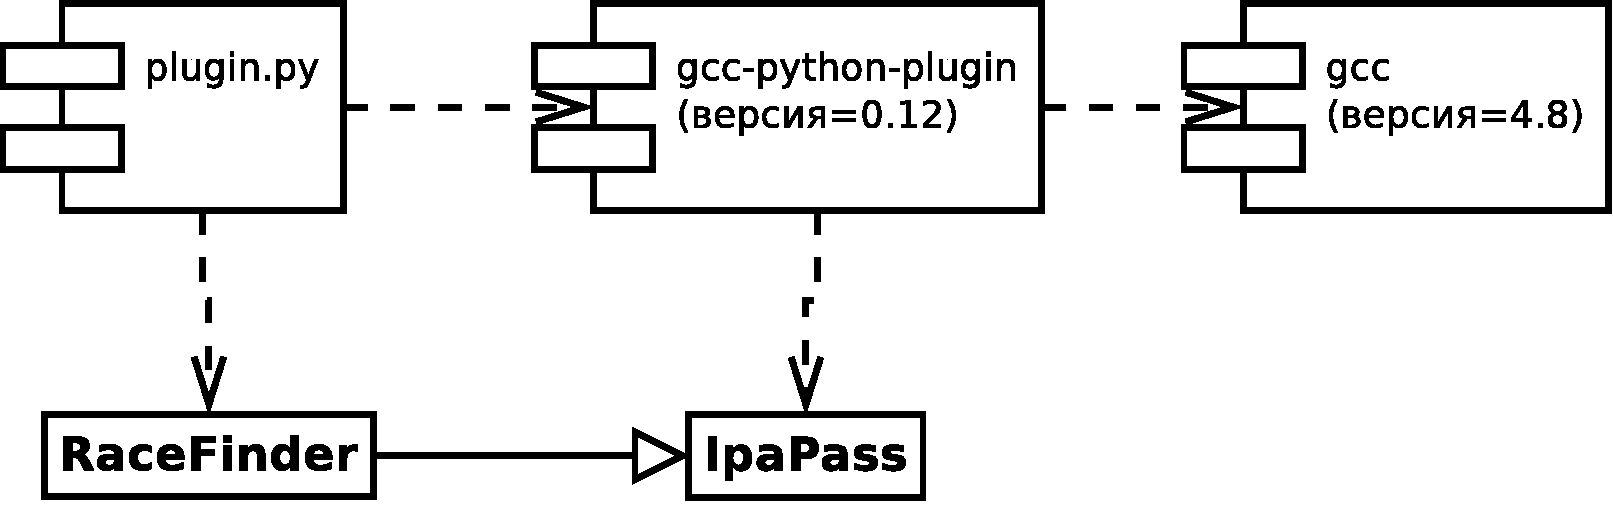
\includegraphics[width=0.8\textwidth]{inc/dia/components}
  \caption{Диаграмма копонентов анализатора}
  \label{fig:components}
\end{figure}

\section{Запуск программы. Формат выходных сообщений}

Для запуска анализатора необходимо выполнить следующую команду к командной строке:
\begin{verbatim}
gcc -fplugin=<path-to-gcc-python-plugin-lib> \
    -fplugin-arg-python=plugin.py \
    -fplugin-arg-python-max-level=<max-level> \
    -fplugin-arg-python-with-main=<with-main> \
    <others>
\end{verbatim}
где:
\begin{itemize}
  \item \textbf{<path-to-gcc-python-plugin-lib>} - путь до библиотеки \textbf{gcc-python-plugon},
  \item \textbf{<max-level>} - максимальное количество раз, которое базовый блок может встретиться в анализируемом пути,
  \item \textbf{<with-main>} - флаг, разрешающий/запрещающий включение в анализ результатов работы главного потока программа, допустимыми значениями которого являются строки $'true'$ и $'false'$,
  \item \textbf{<others>} - обычные параметры, задаваемые при компиляции программы c использованием компилятора \textbf{gcc}.
\end{itemize}

Пример запуска анализатора:
\begin{verbatim}
gcc -fplugin=/home/alex/gcc-python-plugin/python.so \
    -fplugin-arg-python=plugin.py \
    -fplugin-arg-python-max-level=1 \
    -fplugin-arg-python-with-main='true' \
    test.c -lpthread
\end{verbatim}

Сообщение о найденном месте возникновения гонки имеет следующий вид:
\begin{verbatim}
WARNING: Race condition when acccessing the variable <variable-name> (<visibility>) on line <line>
\end{verbatim}
где:
\begin{itemize}
  \item \textbf{<variable-name>} - имя переменной, к которой осуществлялся доступ,
  \item \textbf{<visibility} - область видимости переменной,
  \item \textbf{<line>} - строка, в которой производился доступ.
\end{itemize}

Пример сообщений, выдаваемых анализатором:
\begin{verbatim}
WARNING: Race condition when acccessing the variable buffer (global) on line 37
WARNING: Race condition when acccessing the variable buffer (global) on line 19
\end{verbatim}

\section{Выводы}

бла-бла
